\begin{frame}[label=p12_20260920]{2v1: DATA mass spectra at 40\% and 50\% MC efficiency}
{\small\textbf{Inputs:} \var{Btrk1dR}, \var{Btrk2Pt}}\par\vspace{0.3em}\begin{columns}[T]\column{0.49\textwidth}\centering\textbf{40\%}\par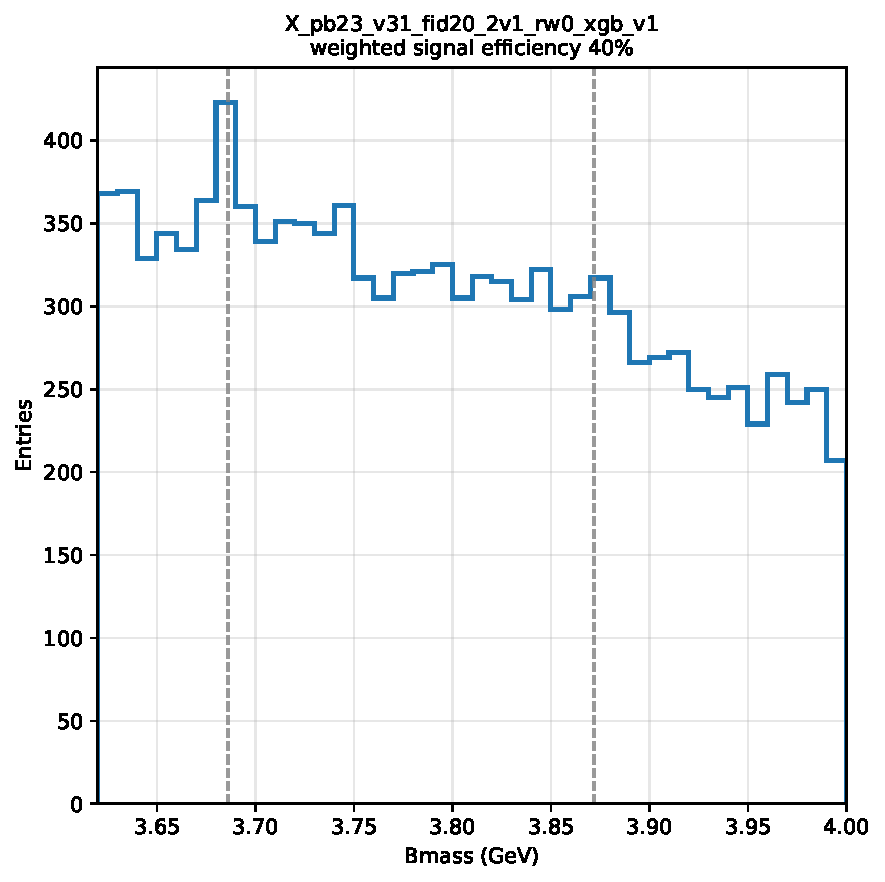
\includegraphics[width=\linewidth,height=0.56\textheight,keepaspectratio]{figures/20260920/2v1_eff40.pdf}\column{0.49\textwidth}\centering\textbf{50\%}\par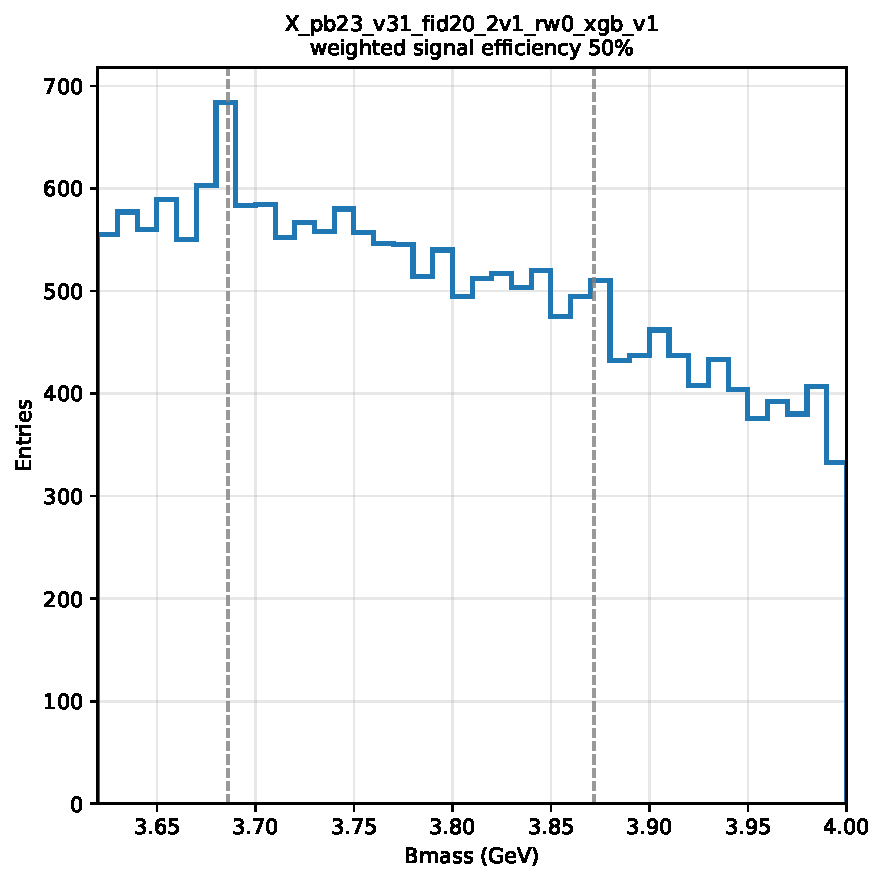
\includegraphics[width=\linewidth,height=0.56\textheight,keepaspectratio]{figures/20260920/2v1_eff50.pdf}\end{columns}\caution{AUC: 0.84197; test AUC: 0.83291; train AUC: 0.84498.}\par\vspace{0.2em}
\caution{Original selected DATA spectra; efficiencies refer to weighted MC after the application selection.}\par\vspace{0.2em}

\end{frame}

\begin{frame}[label=p13_20260920]{2v1: next-input ranking and the selection decision}
{\small Top eight additions by test AUC + baseline. Ranks use unrounded AUC in the full round.}\par
\begin{center}\small\renewcommand{\arraystretch}{1.0}
\begin{tabular}{@{}llrrrr@{}}\toprule
Recipe & Added input & AUC & Rank & test AUC & Rank\\\midrule
3v3 & \var{Btrk1Pt} & 0.90450 & 1 & 0.89177 & 1\\
3v13 & \var{Btktkpt} & 0.90077 & 2 & 0.88902 & 2\\
3v4 & \var{Btrk2dR} & 0.89459 & 3 & 0.88250 & 3\\
\textcolor{positive}{3v5} & \textcolor{positive}{\var{BtrkPtimb}} & \textcolor{positive}{0.88780} & \textcolor{positive}{4} & \textcolor{positive}{0.87474} & \textcolor{positive}{4}\\
3v18 & \var{Balpha} & 0.85722 & 5 & 0.84166 & 5\\
3v15 & \var{Bchi2Prob} & 0.85577 & 6 & 0.84055 & 6\\
3v19 & \var{Bcos_dtheta} & 0.85516 & 7 & 0.83901 & 7\\
3v1 & \var{Bmu1pt} & 0.85379 & 9 & 0.83807 & 8\\
2v1 & \textbf{Baseline (self)} & 0.84197 & 18 & 0.83291 & 15\\
\bottomrule\end{tabular}\end{center}
{\small \textbf{Choose 3v5:} add \var{BtrkPtimb} (test AUC / AUC rank 4 / 4).\par\vspace{0.2em}Higher ranks: \var{Btrk1Pt}, \var{Btktkpt} show positive background--mass association; \var{Btrk2dR} negative association.\par\vspace{0.2em}Initial trigger: the background mass trend in 3v3; later judgments support the other exclusions.}\par
\end{frame}

\begin{frame}[label=p14_20260920]{3v5: DATA mass spectra at 40\% and 50\% MC efficiency}
{\small\textbf{Inputs:} \var{Btrk1dR}, \var{Btrk2Pt}, \var{BtrkPtimb}}\par\vspace{0.3em}\begin{columns}[T]\column{0.49\textwidth}\centering\textbf{40\%}\par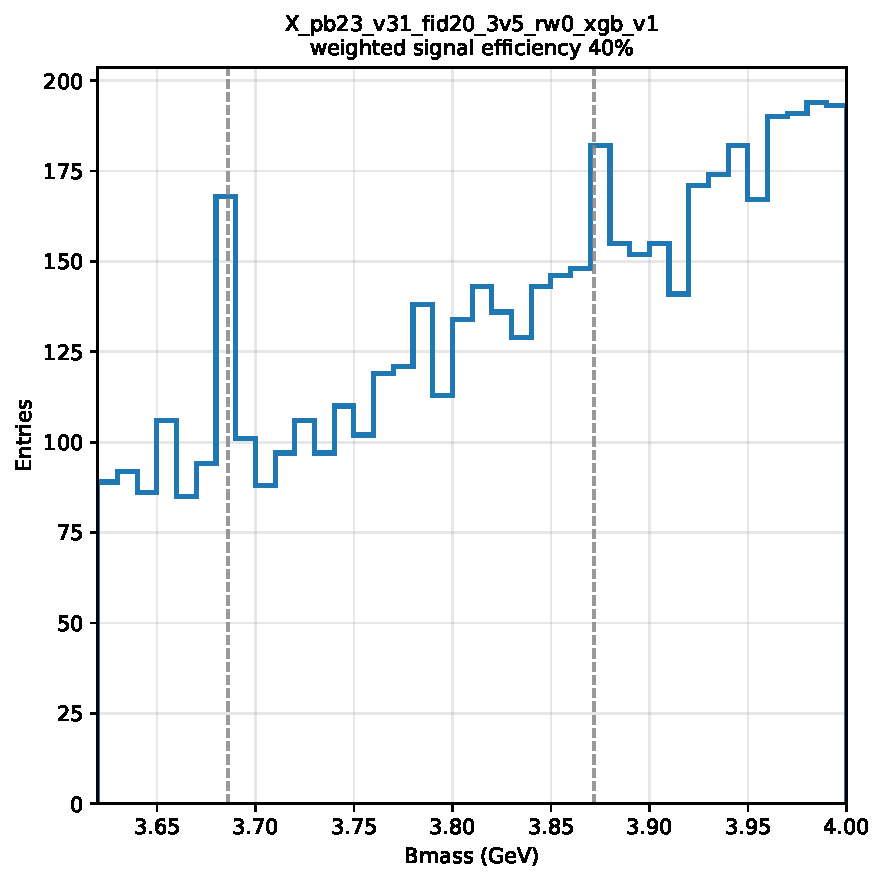
\includegraphics[width=\linewidth,height=0.56\textheight,keepaspectratio]{figures/20260920/3v5_eff40.pdf}\column{0.49\textwidth}\centering\textbf{50\%}\par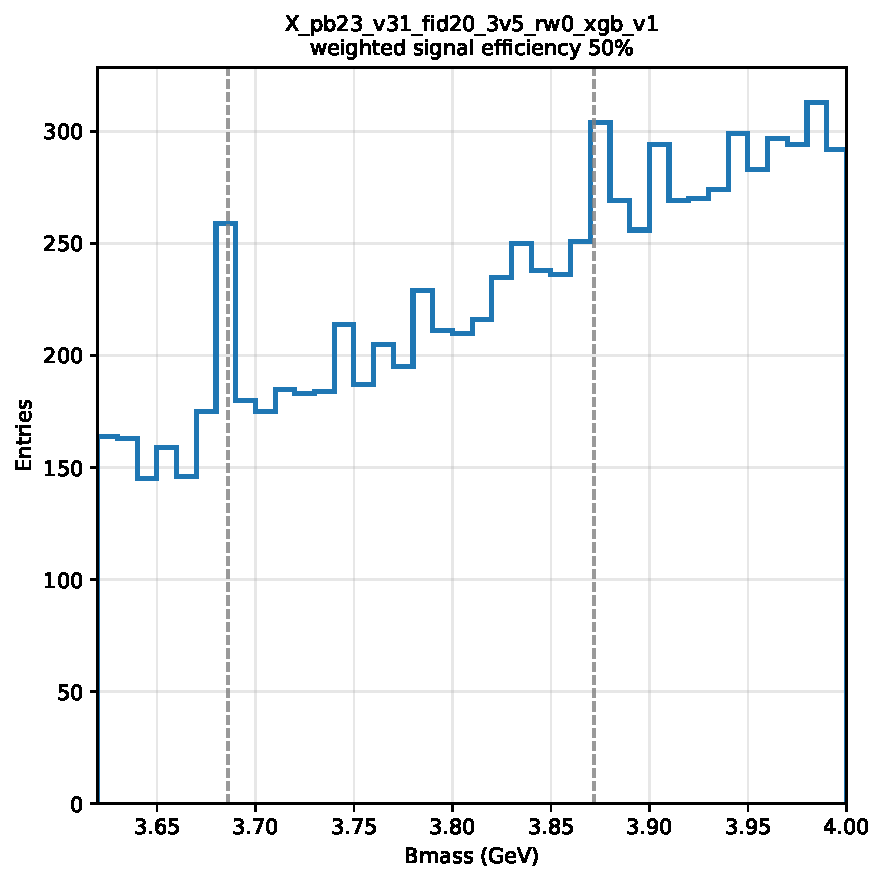
\includegraphics[width=\linewidth,height=0.56\textheight,keepaspectratio]{figures/20260920/3v5_eff50.pdf}\end{columns}\caution{AUC: 0.88780; test AUC: 0.87474; train AUC: 0.89214.}\par\vspace{0.2em}
\caution{Original selected DATA spectra; efficiencies refer to weighted MC after the application selection.}\par\vspace{0.2em}

\end{frame}

\begin{frame}[label=p15_20260920]{3v5: next-input ranking and the selection decision}
{\small Top eight additions by test AUC + baseline. Ranks use unrounded AUC in the full round.}\par
\begin{center}\small\renewcommand{\arraystretch}{1.0}
\begin{tabular}{@{}llrrrr@{}}\toprule
Recipe & Added input & AUC & Rank & test AUC & Rank\\\midrule
4v22 & \var{Btrk1Pt} & 0.90593 & 1 & 0.89173 & 1\\
4v29 & \var{Btktkpt} & 0.90419 & 2 & 0.89070 & 2\\
4v23 & \var{Btrk2dR} & 0.90205 & 3 & 0.88822 & 3\\
4v34 & \var{Balpha} & 0.89775 & 4 & 0.88307 & 4\\
4v31 & \var{Bchi2Prob} & 0.89591 & 6 & 0.88171 & 5\\
\textcolor{positive}{4v35} & \textcolor{positive}{\var{Bcos_dtheta}} & \textcolor{positive}{0.89609} & \textcolor{positive}{5} & \textcolor{positive}{0.88155} & \textcolor{positive}{6}\\
4v20 & \var{Bmu1pt} & 0.89269 & 8 & 0.87786 & 7\\
4v21 & \var{Bmu2pt} & 0.89298 & 7 & 0.87781 & 8\\
3v5 & \textbf{Baseline (self)} & 0.88780 & 17 & 0.87474 & 17\\
\bottomrule\end{tabular}\end{center}
{\small \textbf{Choose 4v35:} add \var{Bcos_dtheta} (test AUC / AUC rank 6 / 5).\par\vspace{0.2em}Ranks 1--3: background mass dependence. \var{Balpha} and \var{Bchi2Prob}: unstable peak changes under tighter cuts.\par\vspace{0.2em}Selection favors background shape and cut stability; no fit-bias claim.}\par
\end{frame}

\begin{frame}[label=p16_20260920]{4v35: DATA mass spectra at 40\% and 50\% MC efficiency}
{\small\textbf{Inputs:} \var{Btrk1dR}, \var{Btrk2Pt}, \var{BtrkPtimb}, \var{Bcos_dtheta}}\par\vspace{0.3em}\begin{columns}[T]\column{0.49\textwidth}\centering\textbf{40\%}\par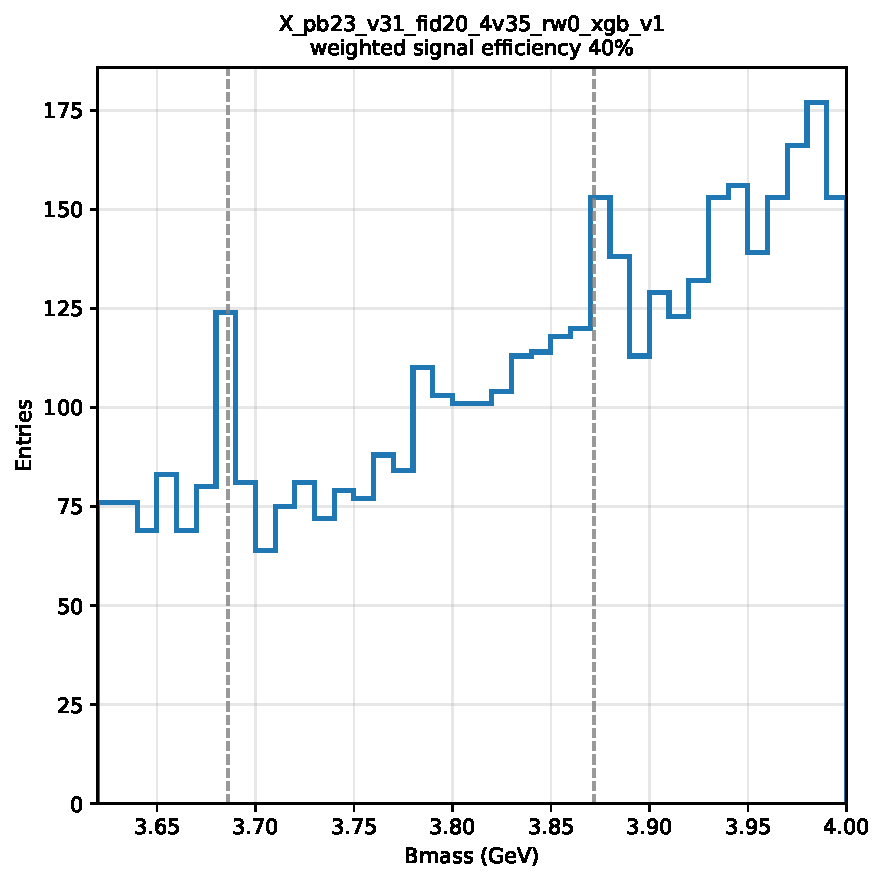
\includegraphics[width=\linewidth,height=0.56\textheight,keepaspectratio]{figures/20260920/4v35_eff40.pdf}\column{0.49\textwidth}\centering\textbf{50\%}\par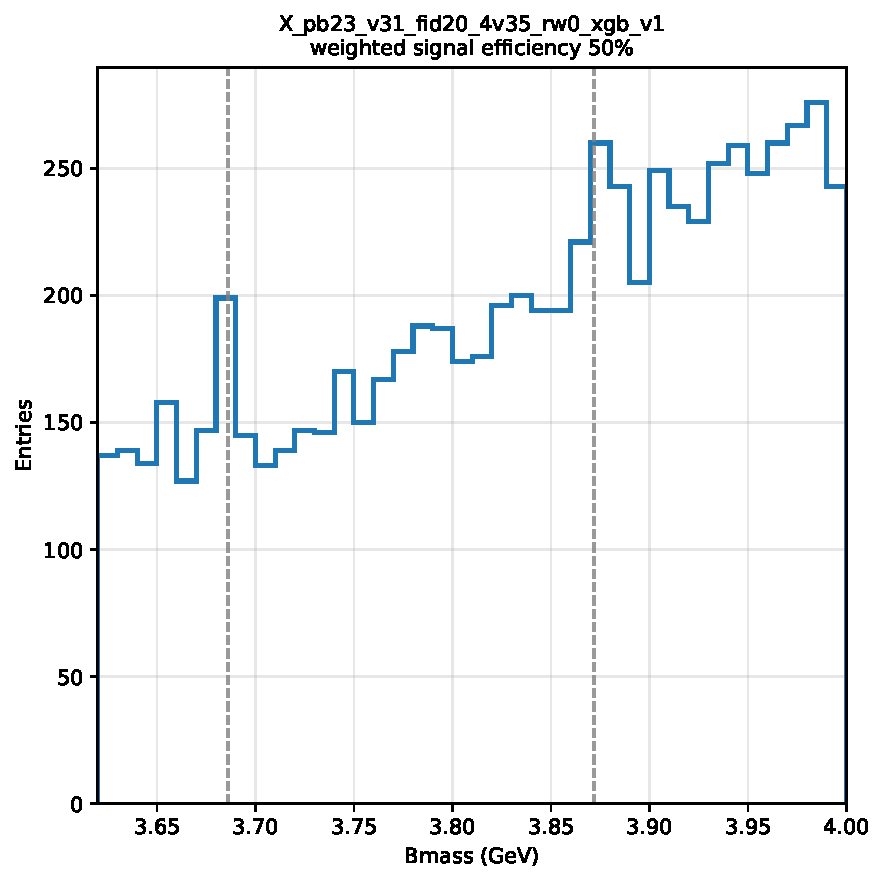
\includegraphics[width=\linewidth,height=0.56\textheight,keepaspectratio]{figures/20260920/4v35_eff50.pdf}\end{columns}\caution{AUC: 0.89609; test AUC: 0.88155; train AUC: 0.90089.}\par\vspace{0.2em}
\caution{Original selected DATA spectra; efficiencies refer to weighted MC after the application selection.}\par\vspace{0.2em}

\end{frame}

\begin{frame}[label=p17_20260920]{4v35: next-input ranking and the selection decision}
{\small Top eight additions by test AUC + baseline. Ranks use unrounded AUC in the full round.}\par
\begin{center}\small\renewcommand{\arraystretch}{1.0}
\begin{tabular}{@{}llrrrr@{}}\toprule
Recipe & Added input & AUC & Rank & test AUC & Rank\\\midrule
5v9 & \var{Btrk1Pt} & 0.91157 & 1 & 0.89646 & 1\\
5v16 & \var{Btktkpt} & 0.90960 & 2 & 0.89481 & 2\\
5v10 & \var{Btrk2dR} & 0.90743 & 3 & 0.89234 & 3\\
5v18 & \var{Bchi2Prob} & 0.90219 & 4 & 0.88678 & 4\\
5v21 & \var{Balpha} & 0.89953 & 5 & 0.88383 & 5\\
5v7 & \var{Bmu1pt} & 0.89928 & 7 & 0.88335 & 6\\
5v8 & \var{Bmu2pt} & 0.89935 & 6 & 0.88299 & 7\\
5v20 & \var{BtktkvProb} & 0.89805 & 14 & 0.88205 & 8\\
4v35 & \textbf{Baseline (self)} & 0.89609 & 16 & 0.88155 & 13\\
\bottomrule\end{tabular}\end{center}
{\small \textbf{Choose 6v13:} add \var{Bmu1pt} and \var{Bmu2pt} together.\par\vspace{0.2em}Ranks 1--3: background mass dependence; ranks 4--5: strict-cut anomalies, suspected MC efficiency limitations.\par\vspace{0.2em}Two-input step approved separately; 6v13 is outside this one-input ranking.}\par
\end{frame}

\begin{frame}[label=p18_20260920]{6v13: DATA mass spectra at 40\% and 50\% MC efficiency}
{\small\textbf{Inputs:} \var{Btrk1dR}, \var{Btrk2Pt}, \var{BtrkPtimb}, \var{Bcos_dtheta}\par \var{Bmu1pt}, \var{Bmu2pt}}\par\vspace{0.3em}\begin{columns}[T]\column{0.49\textwidth}\centering\textbf{40\%}\par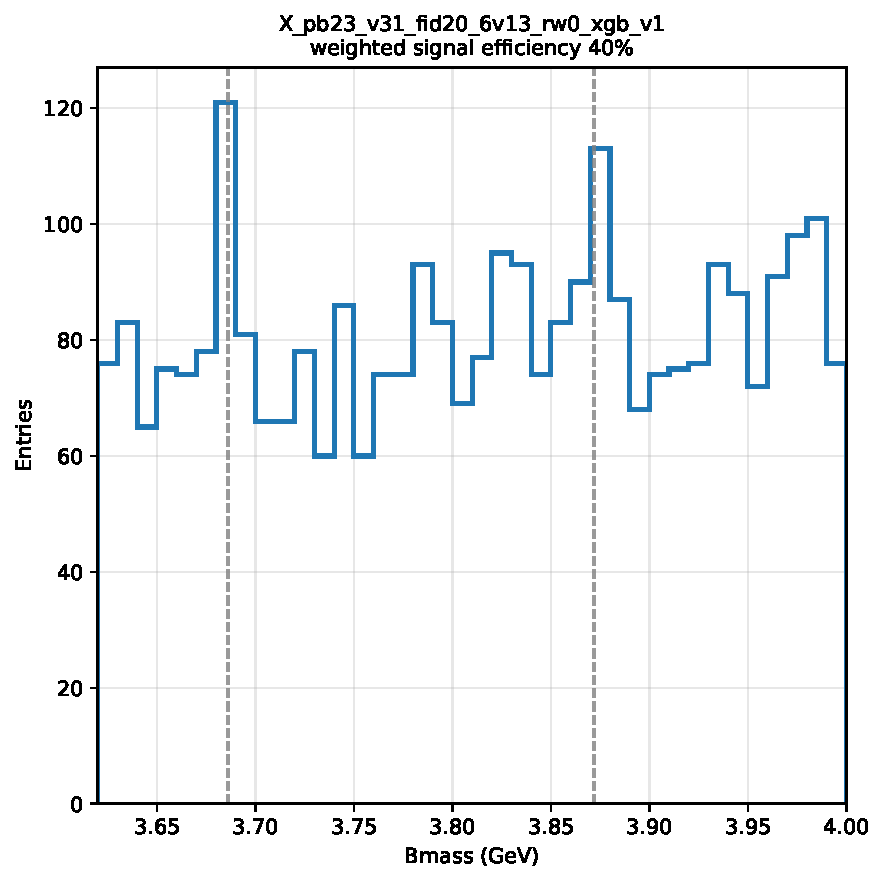
\includegraphics[width=\linewidth,height=0.56\textheight,keepaspectratio]{figures/20260920/6v13_eff40.pdf}\column{0.49\textwidth}\centering\textbf{50\%}\par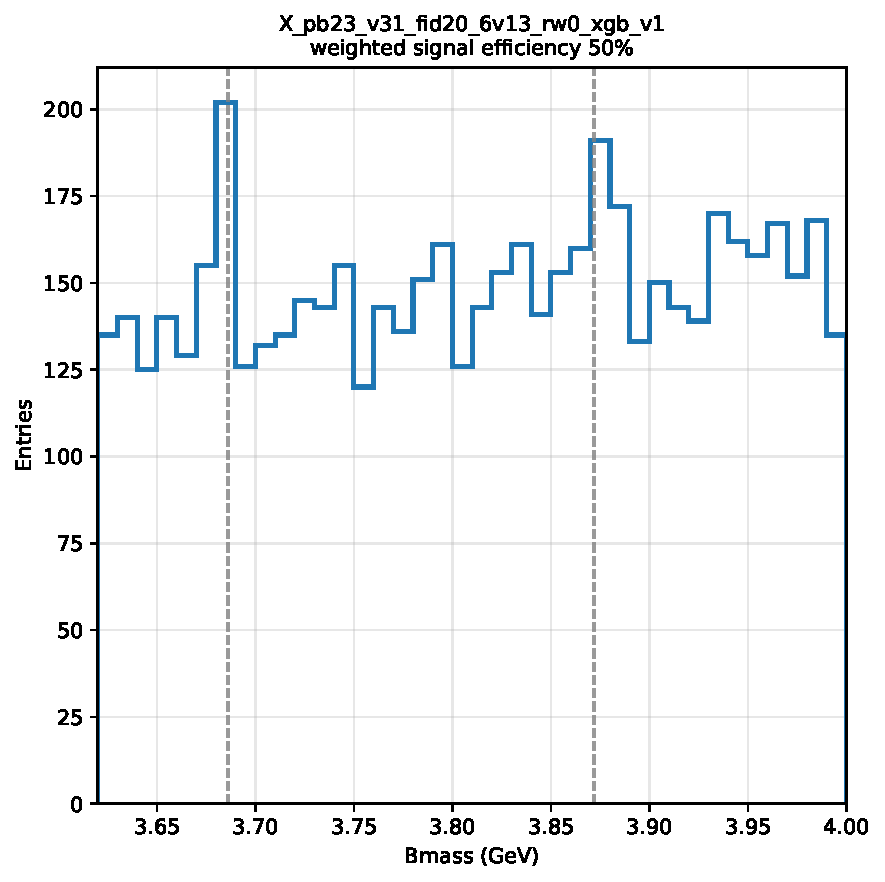
\includegraphics[width=\linewidth,height=0.56\textheight,keepaspectratio]{figures/20260920/6v13_eff50.pdf}\end{columns}\caution{AUC: 0.90434; test AUC: 0.88736; train AUC: 0.90995.}\par\vspace{0.2em}
\caution{Original selected DATA spectra; efficiencies refer to weighted MC after the application selection.}\par\vspace{0.2em}

\end{frame}

\begin{frame}[label=p19_20260920]{6v13: next-input ranking and the selection decision}
{\small Top eight additions by test AUC + baseline. Ranks use unrounded AUC in the full round.}\par
\begin{center}\small\renewcommand{\arraystretch}{1.0}
\begin{tabular}{@{}llrrrr@{}}\toprule
Recipe & Added input & AUC & Rank & test AUC & Rank\\\midrule
7v11 & \var{Btrk1Pt} & 0.91799 & 1 & 0.90093 & 1\\
7v18 & \var{Btktkpt} & 0.91637 & 2 & 0.89907 & 2\\
7v12 & \var{Btrk2dR} & 0.91451 & 3 & 0.89812 & 3\\
7v20 & \var{Bchi2Prob} & 0.90929 & 4 & 0.89192 & 4\\
7v23 & \var{Balpha} & 0.90711 & 5 & 0.88946 & 5\\
\textcolor{positive}{7v17} & \textcolor{positive}{\var{Bujeta}} & \textcolor{positive}{0.90601} & \textcolor{positive}{8} & \textcolor{positive}{0.88793} & \textcolor{positive}{6}\\
7v15 & \var{Btrk1Eta} & 0.90564 & 11 & 0.88779 & 7\\
7v13 & \var{Bmu1eta} & 0.90637 & 6 & 0.88778 & 8\\
6v13 & \textbf{Baseline (self)} & 0.90434 & 14 & 0.88736 & 11\\
\bottomrule\end{tabular}\end{center}
{\small \textbf{Choose 7v17:} add \var{Bujeta} (test AUC / AUC rank 6 / 8).\par\vspace{0.2em}Same exclusions: \var{Btrk1Pt}/\var{Btktkpt} positive, \var{Btrk2dR} negative background--mass association; \var{Bchi2Prob}/\var{Balpha} strict-cut anomalies.\par\vspace{0.2em}The mass-spectrum judgment takes priority over AUC rank.}\par
\end{frame}

\begin{frame}[label=p20_20260920]{7v17: DATA mass spectra at 40\% and 50\% MC efficiency}
{\small\textbf{Inputs:} \var{Btrk1dR}, \var{Btrk2Pt}, \var{BtrkPtimb}, \var{Bcos_dtheta}\par \var{Bmu1pt}, \var{Bmu2pt}, \var{Bujeta}}\par\vspace{0.3em}\begin{columns}[T]\column{0.49\textwidth}\centering\textbf{40\%}\par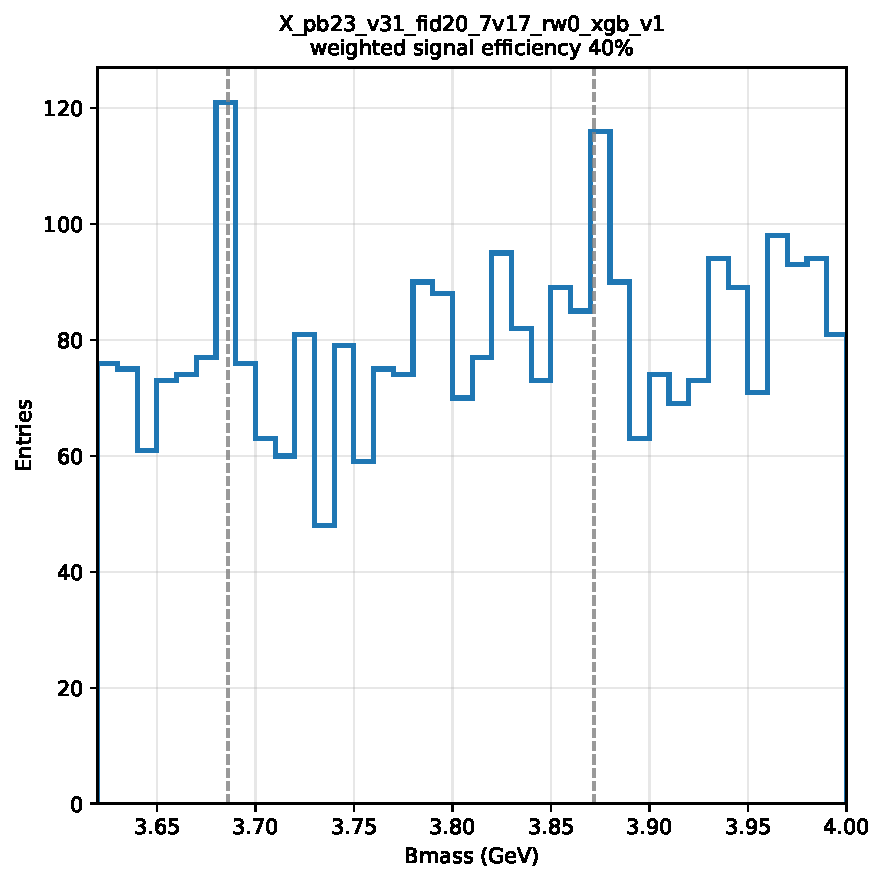
\includegraphics[width=\linewidth,height=0.56\textheight,keepaspectratio]{figures/20260920/7v17_eff40.pdf}\column{0.49\textwidth}\centering\textbf{50\%}\par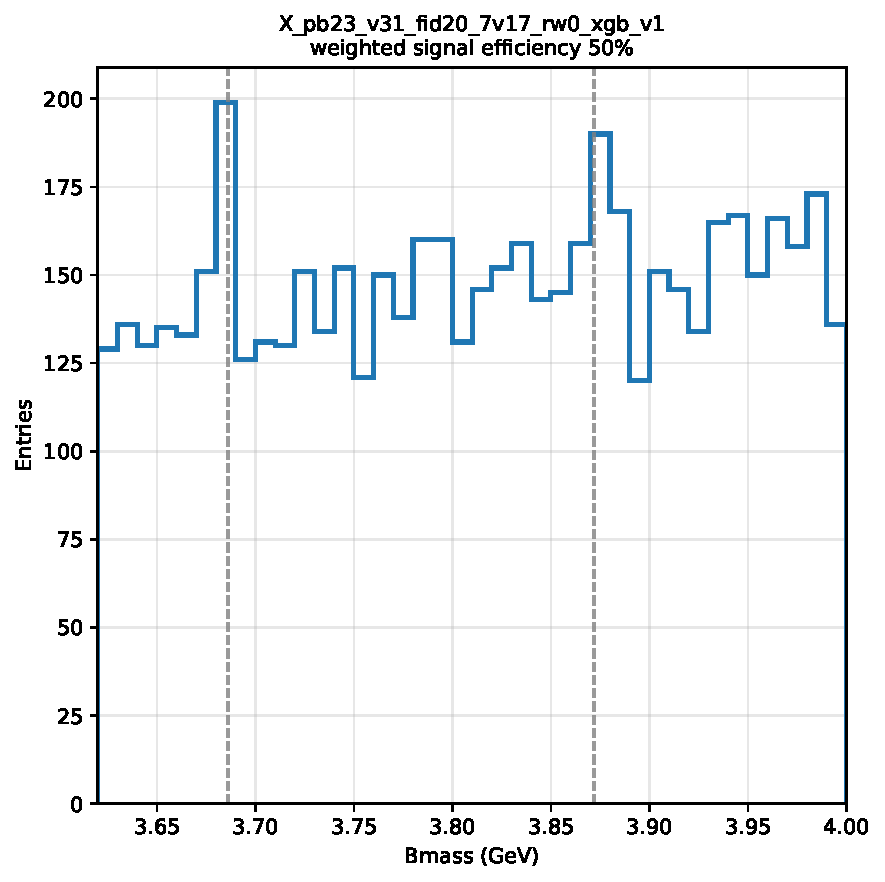
\includegraphics[width=\linewidth,height=0.56\textheight,keepaspectratio]{figures/20260920/7v17_eff50.pdf}\end{columns}\caution{AUC: 0.90601; test AUC: 0.88793; train AUC: 0.91198.}\par\vspace{0.2em}
\caution{Original selected DATA spectra; efficiencies refer to weighted MC after the application selection.}\par\vspace{0.2em}

\end{frame}

\begin{frame}[label=p21_20260920]{7v17: next-input ranking and the selection decision}
{\small Top eight additions by test AUC + baseline. Ranks use unrounded AUC in the full round.}\par
\begin{center}\small\renewcommand{\arraystretch}{1.0}
\begin{tabular}{@{}llrrrr@{}}\toprule
Recipe & Added input & AUC & Rank & test AUC & Rank\\\midrule
8v23 & \var{Btrk1Pt} & 0.91913 & 1 & 0.90079 & 1\\
8v29 & \var{Btktkpt} & 0.91765 & 2 & 0.89927 & 2\\
8v24 & \var{Btrk2dR} & 0.91552 & 3 & 0.89829 & 3\\
8v31 & \var{Bchi2Prob} & 0.91070 & 4 & 0.89231 & 4\\
8v34 & \var{Balpha} & 0.90903 & 5 & 0.89031 & 5\\
8v30 & \var{Btktketa} & 0.90672 & 8 & 0.88843 & 6\\
8v25 & \var{Bmu1eta} & 0.90710 & 7 & 0.88818 & 7\\
8v32 & \var{BujvProb} & 0.90724 & 6 & 0.88793 & 9\\
\textcolor{positive}{7v17} & \textcolor{positive}{\textbf{Baseline (self)}} & \textcolor{positive}{0.90601} & \textcolor{positive}{13} & \textcolor{positive}{0.88793} & \textcolor{positive}{8}\\
\bottomrule\end{tabular}\end{center}
{\small \textbf{Retain 7v17:} no additional input is adopted.\par\vspace{0.2em}Ranks 1--5 retain the preceding concerns. \var{Btktketa} additionally suppresses the observed X feature, raising an MC-efficiency concern.\par\vspace{0.2em}Remaining test AUC gains do not motivate another step in the human choice.}\par
\end{frame}

\begin{frame}[label=p22_20260920]{Interim conclusion: 7v17 is the preferred recipe in this study}

\begin{center}\small\renewcommand{\arraystretch}{1.0}
\begin{tabular}{@{}lrrr@{}}\toprule
Recipe & train AUC & test AUC & AUC\\\midrule
2v1 & 0.84498 & 0.83291 & 0.84197\\
3v5 & 0.89214 & 0.87474 & 0.88780\\
4v35 & 0.90089 & 0.88155 & 0.89609\\
6v13 & 0.90995 & 0.88736 & 0.90434\\
7v17 & 0.91198 & 0.88793 & 0.90601\\
\bottomrule\end{tabular}\end{center}
\begin{itemize}\small\item AUC gains are considered together with background mass shape and stability under tighter cuts.\item The selected seven inputs are \var{Btrk1dR}, \var{Btrk2Pt}, \var{BtrkPtimb}, \var{Bcos_dtheta}, \var{Bmu1pt}, \var{Bmu2pt}, \var{Bujeta}.\item Further additions are not adopted; the current choice is \textbf{7v17}.\end{itemize}\caution{Preferred within the current allowed-variable study and MC assumption; final nominal selection and working point remain open.}\par\vspace{0.2em}
\end{frame}

